% -----------------------------------------------------------------------------
%                                     HEADER                                    
% -----------------------------------------------------------------------------
\documentclass[a4paper, 10pt]{article}
\usepackage{jheppub}
\usepackage[T1]{fontenc}
\usepackage{colortbl,xcolor,float}
\definecolor{orange}{rgb}{1,0.5,0}
% -----------------------------------------------------------------------------
%                                   COVER PAGE                                  
% -----------------------------------------------------------------------------
\title{{\includegraphics[scale=.4]{logo.png}}\ The LaTeX report}

\author{Generated by bkailasa on 17 January 2020, 11:06:44}

\abstract{
  This report has been generated automatically
  by {\sc MadAnalysis} 5.\\$~$\\ 
  Please cite:\\ 
  \begin{quote}
    \textbf{E.~Conte, B.~Fuks and G.~Serret},\\ 
    \textit{MadAnalysis 5, A User-Friendly
    Framework for Collider Phenomenology},\\ 
    Comput. Phys. Commun. {\bf 184} (2013) 222-256,\\
    arXiv:1206.1599 [hep-ph].\\ 
  \end{quote}
  To contact us:\\ 
  \begin{quote}
    \textbf{http://madanalysis.irmp.ucl.ac.be}\\
    \textbf{ma5team@iphc.cnrs.fr}\\
  \end{quote}
}

% -----------------------------------------------------------------------------
%                                 BEGIN DOCUMENT                                
% -----------------------------------------------------------------------------
\begin{document}
\maketitle
\flushbottom

% -----------------------------------------------------------------------------
%                                 SECTION Setup                                 
% -----------------------------------------------------------------------------
\newpage
\section{ Setup}

\subsection{ Command history}

\texttt{ma5>import /\-afs/\-cern.ch/\-work/\-b/\-bkailasa/\-MCGens/\-madgraph/\-MG5\_aMC\_v2\_6\_7/\-PROC\_Tutorial\_UFO\_0/\-bin/\-internal/\-ufomodel\\
}
\texttt{ }\texttt{ }\texttt{ma5>import /\-afs/\-cern.ch/\-work/\-b/\-bkailasa/\-MCGens/\-madgraph/\-MG5\_aMC\_v2\_6\_7/\-PROC\_Tutorial\_UFO\_0/\-Events/\-run\_01/\-unweighted\_events.lhe.gz as unweighted\_events\\
}
\texttt{ }\texttt{ }\texttt{ma5>define vl = 12 14 16\\
}
\texttt{ }\texttt{ }\texttt{ma5>define vl~ = -16 -14 -12\\
}
\texttt{ }\texttt{ }\texttt{ma5>define invisible = ve ve~ vm vm~ vt vt~ vl vl~\\
}
\texttt{ }\texttt{ }\texttt{ma5>set main.graphic\_render = root\\
}
\texttt{ }\texttt{ }\texttt{ma5>plot THT   40 0 500 [logY]\\
}
\texttt{ }\texttt{ }\texttt{ma5>plot MET   40 0 500 [logY]\\
}
\texttt{ }\texttt{ }\texttt{ma5>plot SQRTS 40 0 500 [logY]\\
}
\texttt{ }\texttt{ }\texttt{ma5>plot  PT(uv[1]) 40 0  500 [logY interstate]\\
}
\texttt{ }\texttt{ }\texttt{ma5>plot ETA(uv[1]) 40 -10 10 [logY interstate]\\
}
\texttt{ }\texttt{ }\texttt{ma5>plot  PT(uv~[1]) 40 0  500 [logY]\\
}
\texttt{ }\texttt{ }\texttt{ma5>plot ETA(uv~[1]) 40 -10 10 [logY]\\
}
\texttt{ }\texttt{ }\texttt{ma5>plot M(uv[1] uv~[1]) 40 0  500 [logY allstate]\\
}
\texttt{ }\texttt{ }\texttt{ma5>plot DELTAR(uv[1],uv~[1]) 40 0 10 [logY allstate]\\
}
\texttt{ }\texttt{ }\texttt{ma5>plot  PT(c[1]) 40 0  500 [logY]\\
}
\texttt{ }\texttt{ }\texttt{ma5>plot ETA(c[1]) 40 -10 10 [logY]\\
}
\texttt{ }\texttt{ }\texttt{ma5>plot  PT(p1[1]) 40 0  500 [logY]\\
}
\texttt{ }\texttt{ }\texttt{ma5>plot ETA(p1[1]) 40 -10 10 [logY]\\
}
\texttt{ }\texttt{ }\texttt{ma5>plot  PT(uv~[1]) 40 0  500 [logY]\\
}
\texttt{ }\texttt{ }\texttt{ma5>plot ETA(uv~[1]) 40 -10 10 [logY]\\
}
\texttt{ }\texttt{ }\texttt{ma5>plot M(c[1] p1[1]) 40 0  500 [logY ]\\
}
\texttt{ }\texttt{ }\texttt{ma5>plot M(c[1] p1[1] uv~[1]) 40 0  500 [logY ]\\
}
\texttt{ }\texttt{ }\texttt{ma5>plot M(c[1] uv~[1]) 40 0  500 [logY ]\\
}
\texttt{ }\texttt{ }\texttt{ma5>plot M(p1[1] uv~[1]) 40 0  500 [logY ]\\
}
\texttt{ }\texttt{ }\texttt{ma5>plot DELTAR(c[1],p1[1]) 40 0 10 [logY ]\\
}
\texttt{ }\texttt{ }\texttt{ma5>plot DELTAR(c[1],uv~[1]) 40 0 10 [logY ]\\
}
\texttt{ }\texttt{ }\texttt{ma5>plot DELTAR(p1[1],uv~[1]) 40 0 10 [logY ]\\
}
\texttt{ }\texttt{ }\texttt{ma5>submit /\-afs/\-cern.ch/\-work/\-b/\-bkailasa/\-MCGens/\-madgraph/\-MG5\_aMC\_v2\_6\_7/\-PROC\_Tutorial\_UFO\_0/\-MA5\_PARTON\_ANALYSIS\_analysis1\\
}
\texttt{ }\texttt{ }\subsection{ Configuration}

\begin{itemize}
  \item MadAnalysis version 1.8.31 (2019/\-11/\-06).
   \item Histograms given for an integrated luminosity of \textcolor{blue}{10}\textcolor{blue}{ fb}$^{\textcolor{blue}{-1}}$\textcolor{blue}{.}
\textcolor{blue}{}
\end{itemize}
% -----------------------------------------------------------------------------
%                                SECTION Datasets                               
% -----------------------------------------------------------------------------
\newpage
\section{ Datasets}

\subsection{ unweighted\_events}

\begin{itemize}
  \item Sample consisting of: \textcolor{blue}{signal}  events.
   \item Generated events: \textcolor{blue}{10000 }  events.
   \item Normalization to the luminosity: \textcolor{blue}{2982}\textcolor{blue}{ +/\-- }\textcolor{blue}{6 }  events.
   \item Ratio (event weight): \textcolor{blue}{0.3 } .  
 
\end{itemize}
\begin{table}[H]
  \begin{center}
    \begin{tabular}{|m{55.0mm}|m{25.0mm}|m{30.0mm}|m{30.0mm}|}
      \hline
      {\cellcolor{yellow}         Path to the event file}& {\cellcolor{yellow}         Nr. of events}& {\cellcolor{yellow}         Cross section (pb)}& {\cellcolor{yellow}         Negative wgts (\%)}\\
      \hline
      {\cellcolor{white}          PROC\_Tutorial\_UFO\_0/\-Events/\-run\_01/\-unweighted\_events.lhe.gz}& {\cellcolor{white}          10000}& {\cellcolor{white}          0.298 @ 0.18\%}& {\cellcolor{white}          0.0}\\
\hline
    \end{tabular}
  \end{center}
\end{table}

% -----------------------------------------------------------------------------
%                            SECTION Histos and cuts                            
% -----------------------------------------------------------------------------
\newpage
\section{ Histos and cuts}

\subsection{ Histogram 1}

\textbf{* Plot: THT}\\
   \begin{table}[H]
  \begin{center}
    \begin{tabular}{|m{23.0mm}|m{23.0mm}|m{18.0mm}|m{19.0mm}|m{19.0mm}|m{19.0mm}|m{19.0mm}|}
      \hline
      {\cellcolor{yellow}         Dataset}& {\cellcolor{yellow}         Integral}& {\cellcolor{yellow}         Entries per event}& {\cellcolor{yellow}         Mean}& {\cellcolor{yellow}         RMS}& {\cellcolor{yellow}         \% underflow}& {\cellcolor{yellow}         \% overflow}\\
      \hline
      {\cellcolor{white}         unweighted\_events}& {\cellcolor{white}         2982}& {\cellcolor{white}         1.0}& {\cellcolor{white}         206.941}& {\cellcolor{white}         115.3}& {\cellcolor{green}         0.0}& {\cellcolor{green}         2.17}\\
\hline
    \end{tabular}
  \end{center}
\end{table}

\begin{figure}[H]
  \begin{center}
    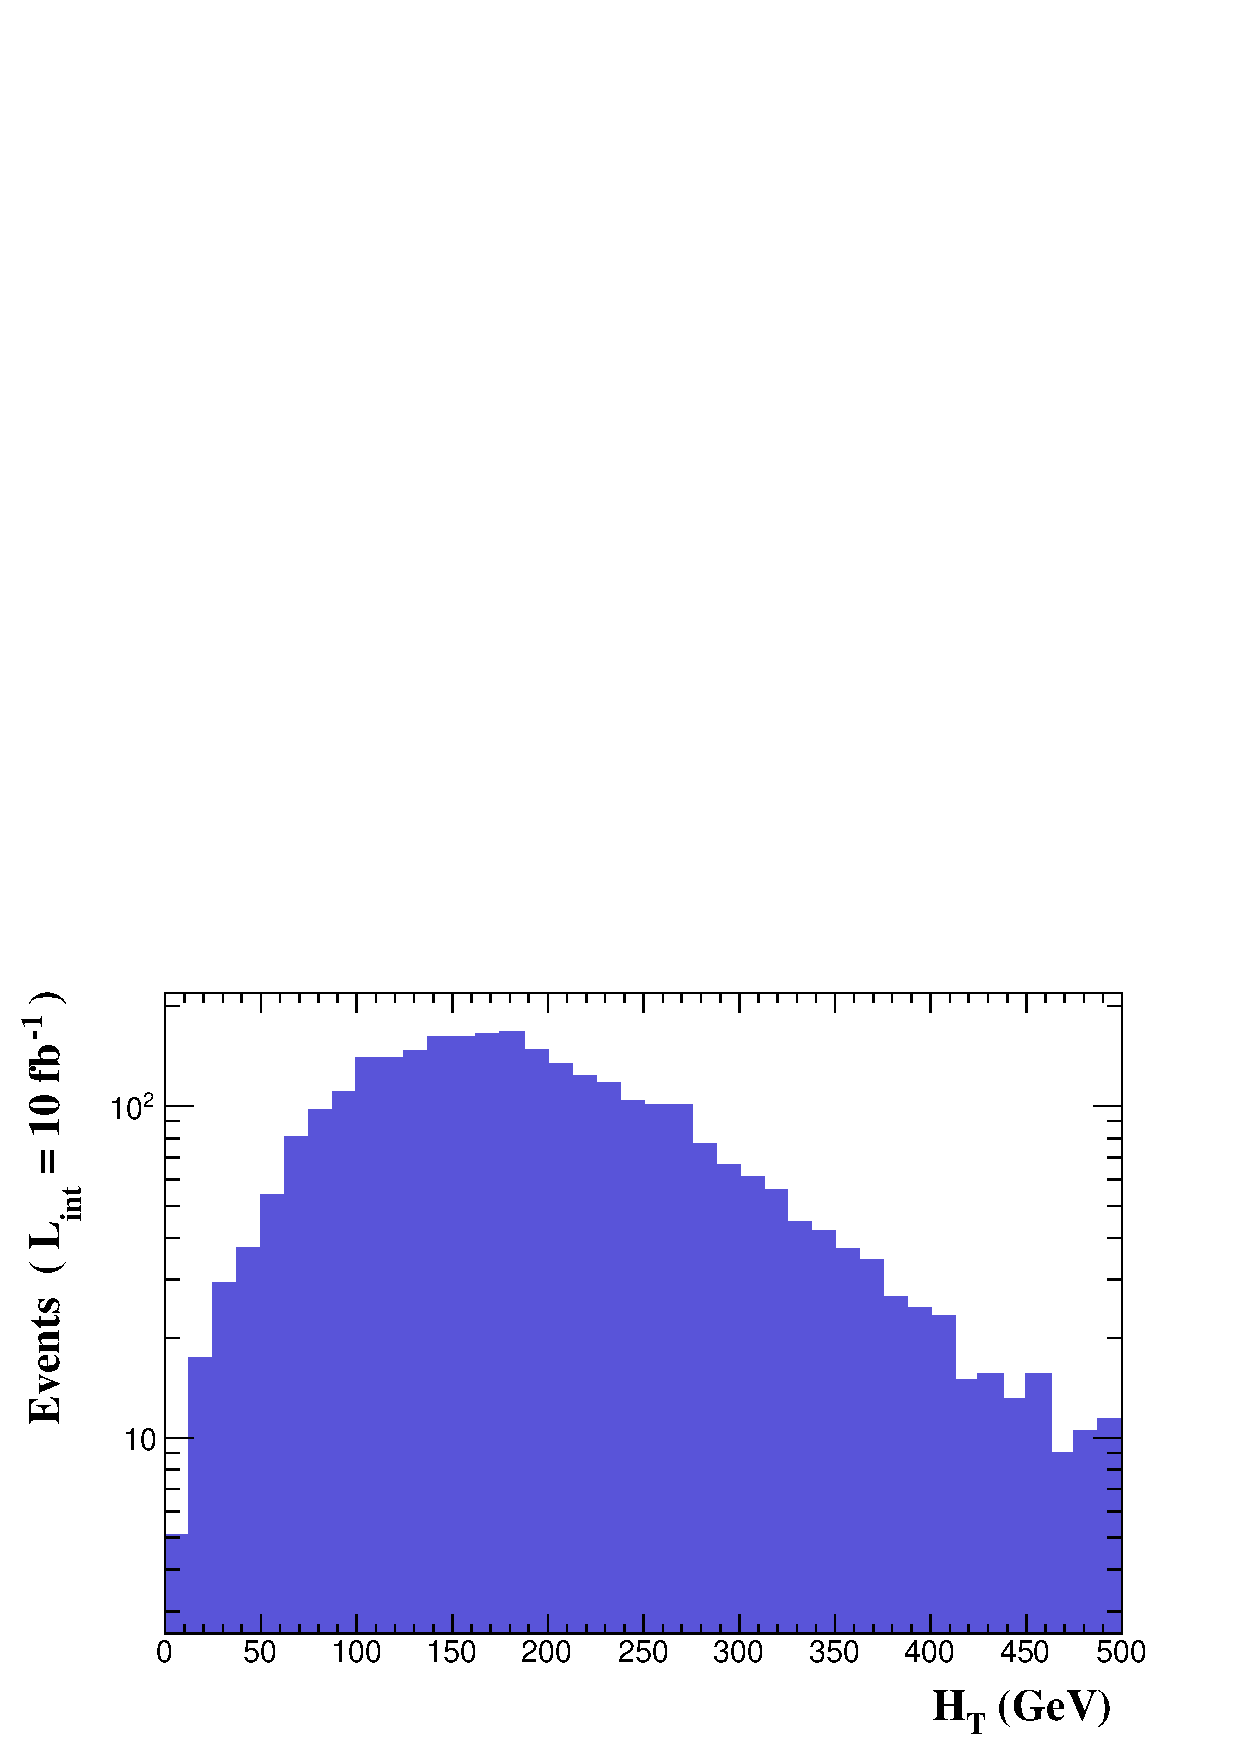
\includegraphics[scale=0.45]{selection_0.png}\\
\caption{   }
  \end{center}
\end{figure}
      \newpage
\subsection{ Histogram 2}

\textbf{* Plot: MET}\\
   \begin{table}[H]
  \begin{center}
    \begin{tabular}{|m{23.0mm}|m{23.0mm}|m{18.0mm}|m{19.0mm}|m{19.0mm}|m{19.0mm}|m{19.0mm}|}
      \hline
      {\cellcolor{yellow}         Dataset}& {\cellcolor{yellow}         Integral}& {\cellcolor{yellow}         Entries per event}& {\cellcolor{yellow}         Mean}& {\cellcolor{yellow}         RMS}& {\cellcolor{yellow}         \% underflow}& {\cellcolor{yellow}         \% overflow}\\
      \hline
      {\cellcolor{white}         unweighted\_events}& {\cellcolor{white}         2982}& {\cellcolor{white}         1.0}& {\cellcolor{white}         4.43006e-09}& {\cellcolor{white}         3.146e-09}& {\cellcolor{green}         0.0}& {\cellcolor{green}         0.0}\\
\hline
    \end{tabular}
  \end{center}
\end{table}

\begin{figure}[H]
  \begin{center}
    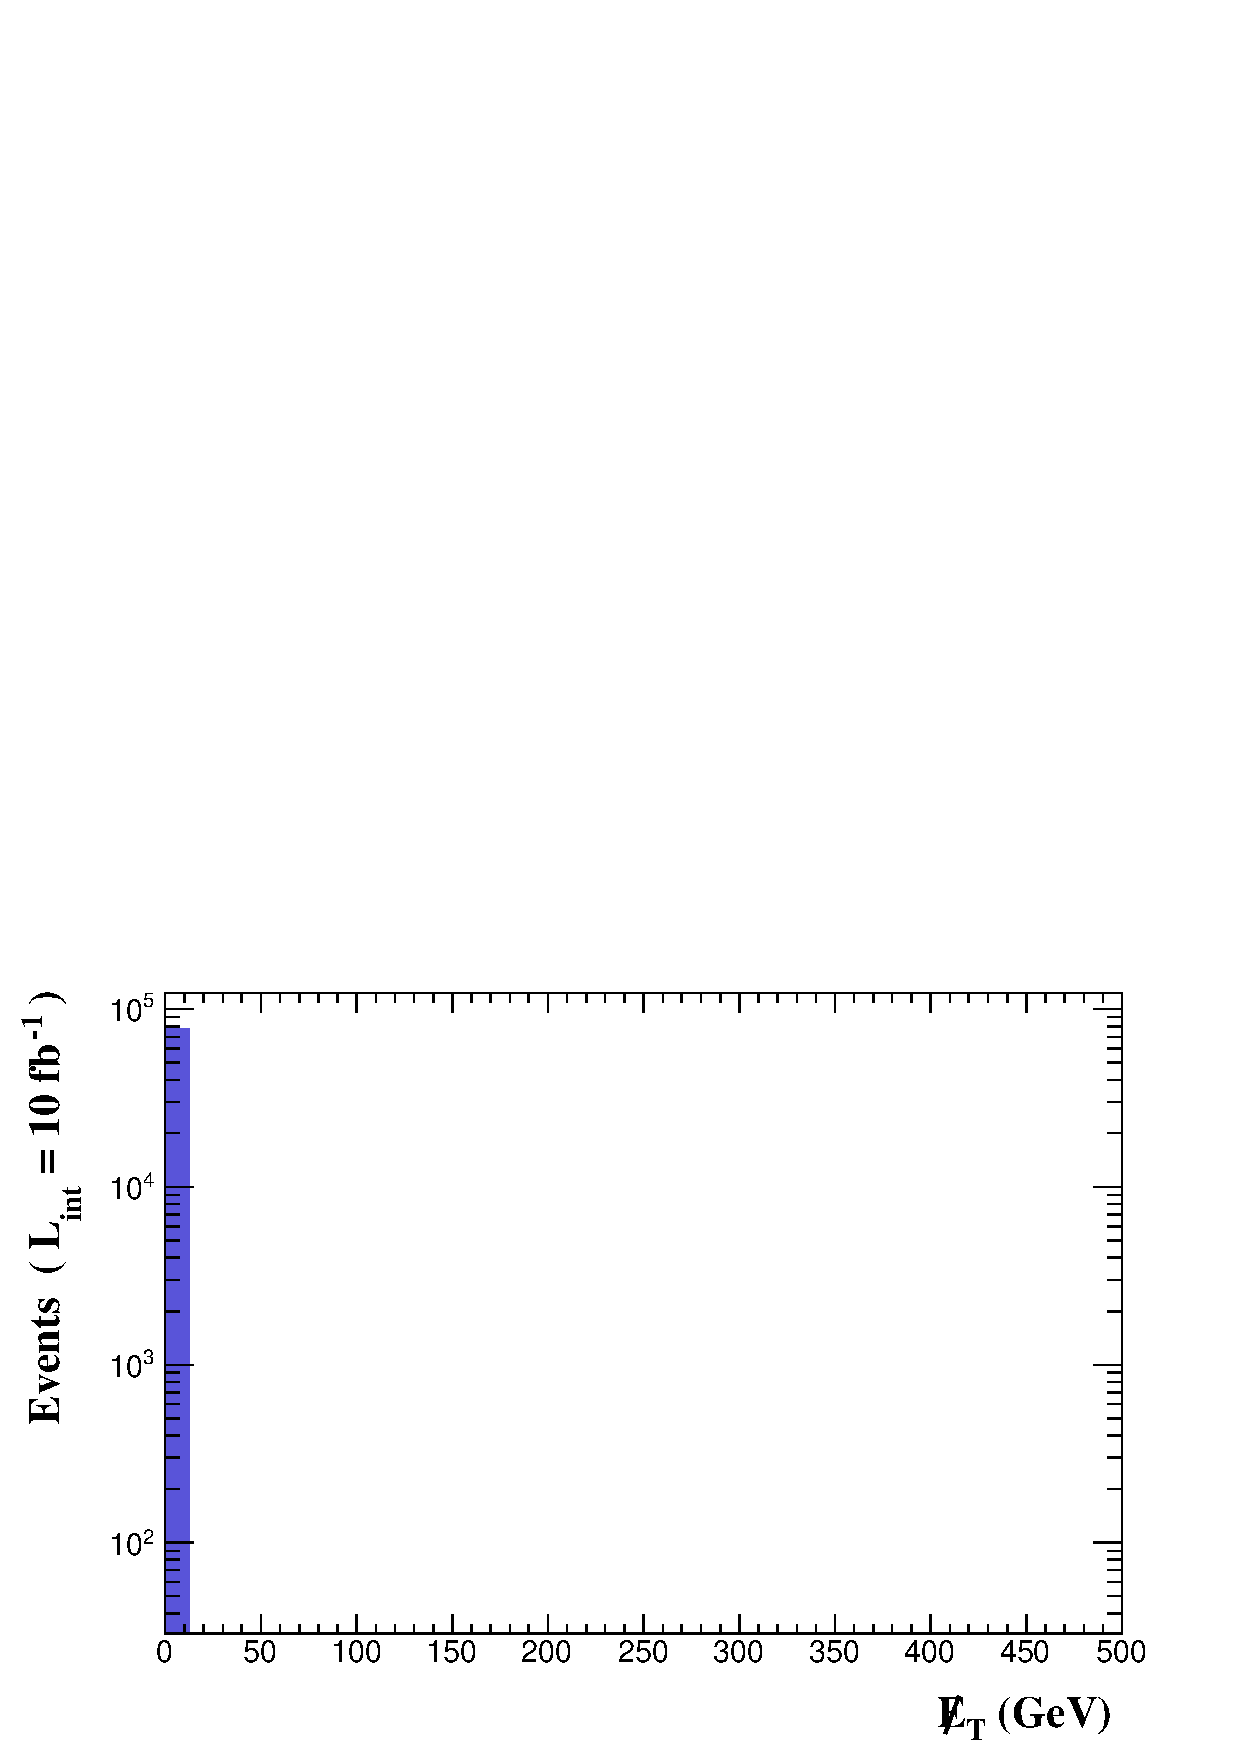
\includegraphics[scale=0.45]{selection_1.png}\\
\caption{   }
  \end{center}
\end{figure}
      \newpage
\subsection{ Histogram 3}

\textbf{* Plot: SQRTS}\\
   \begin{table}[H]
  \begin{center}
    \begin{tabular}{|m{23.0mm}|m{23.0mm}|m{18.0mm}|m{19.0mm}|m{19.0mm}|m{19.0mm}|m{19.0mm}|}
      \hline
      {\cellcolor{yellow}         Dataset}& {\cellcolor{yellow}         Integral}& {\cellcolor{yellow}         Entries per event}& {\cellcolor{yellow}         Mean}& {\cellcolor{yellow}         RMS}& {\cellcolor{yellow}         \% underflow}& {\cellcolor{yellow}         \% overflow}\\
      \hline
      {\cellcolor{white}         unweighted\_events}& {\cellcolor{white}         2982}& {\cellcolor{white}         1.0}& {\cellcolor{white}         1122.71}& {\cellcolor{white}         302.3}& {\cellcolor{red}         0.0}& {\cellcolor{red}         100.0}\\
\hline
    \end{tabular}
  \end{center}
\end{table}

\begin{figure}[H]
  \begin{center}
    \includegraphics[scale=0.45]{selection_2.png}\\
\caption{   }
  \end{center}
\end{figure}
      \newpage
\subsection{ Histogram 4}

\textbf{* Plot: PT ( uv[1] ) }\\
   \begin{table}[H]
  \begin{center}
    \begin{tabular}{|m{23.0mm}|m{23.0mm}|m{18.0mm}|m{19.0mm}|m{19.0mm}|m{19.0mm}|m{19.0mm}|}
      \hline
      {\cellcolor{yellow}         Dataset}& {\cellcolor{yellow}         Integral}& {\cellcolor{yellow}         Entries per event}& {\cellcolor{yellow}         Mean}& {\cellcolor{yellow}         RMS}& {\cellcolor{yellow}         \% underflow}& {\cellcolor{yellow}         \% overflow}\\
      \hline
      {\cellcolor{white}         unweighted\_events}& {\cellcolor{white}         2982}& {\cellcolor{white}         1.0}& {\cellcolor{white}         251.371}& {\cellcolor{white}         157.0}& {\cellcolor{orange}         0.0}& {\cellcolor{orange}         6.98}\\
\hline
    \end{tabular}
  \end{center}
\end{table}

\begin{figure}[H]
  \begin{center}
    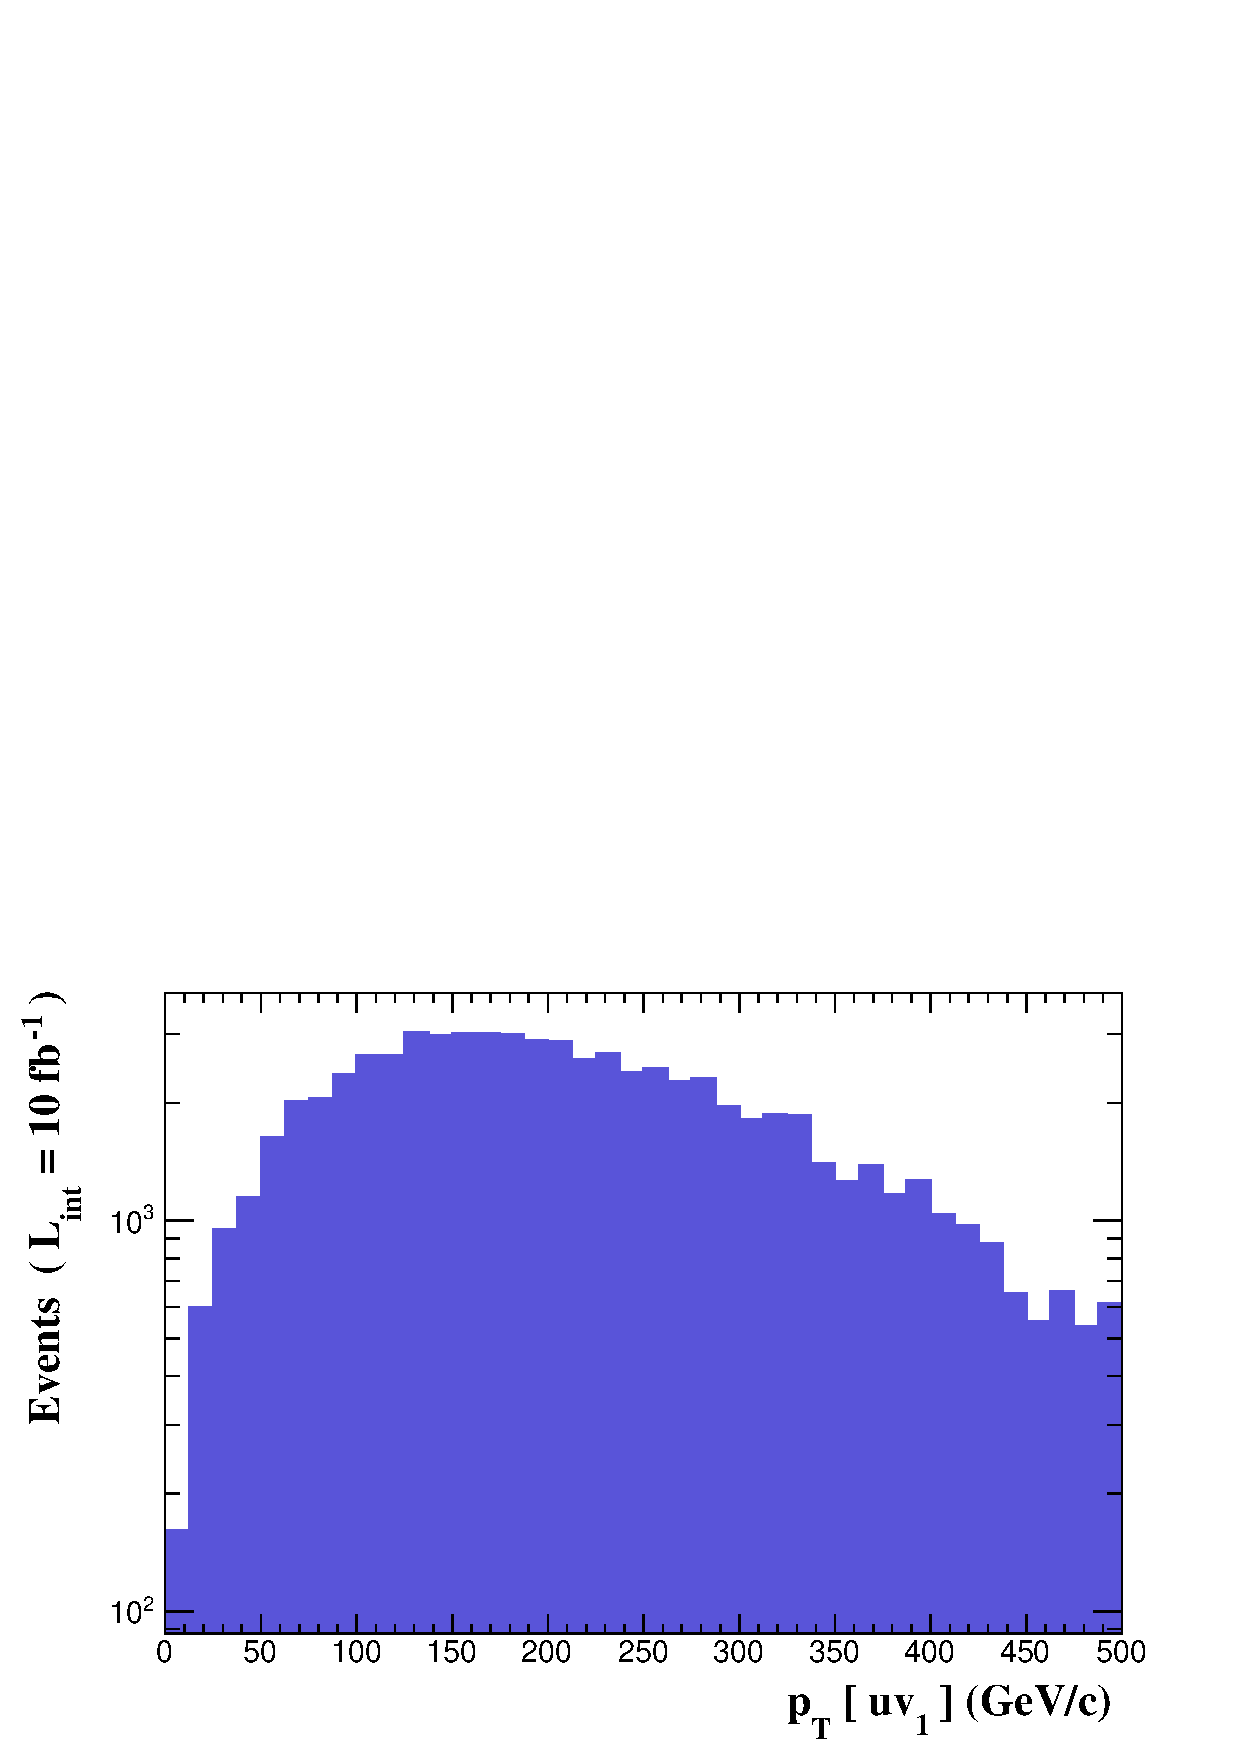
\includegraphics[scale=0.45]{selection_3.png}\\
\caption{   }
  \end{center}
\end{figure}
      \newpage
\subsection{ Histogram 5}

\textbf{* Plot: ETA ( uv[1] ) }\\
   \begin{table}[H]
  \begin{center}
    \begin{tabular}{|m{23.0mm}|m{23.0mm}|m{18.0mm}|m{19.0mm}|m{19.0mm}|m{19.0mm}|m{19.0mm}|}
      \hline
      {\cellcolor{yellow}         Dataset}& {\cellcolor{yellow}         Integral}& {\cellcolor{yellow}         Entries per event}& {\cellcolor{yellow}         Mean}& {\cellcolor{yellow}         RMS}& {\cellcolor{yellow}         \% underflow}& {\cellcolor{yellow}         \% overflow}\\
      \hline
      {\cellcolor{white}         unweighted\_events}& {\cellcolor{white}         2982}& {\cellcolor{white}         1.0}& {\cellcolor{white}         -0.0206212}& {\cellcolor{white}         1.685}& {\cellcolor{green}         0.0}& {\cellcolor{green}         0.0}\\
\hline
    \end{tabular}
  \end{center}
\end{table}

\begin{figure}[H]
  \begin{center}
    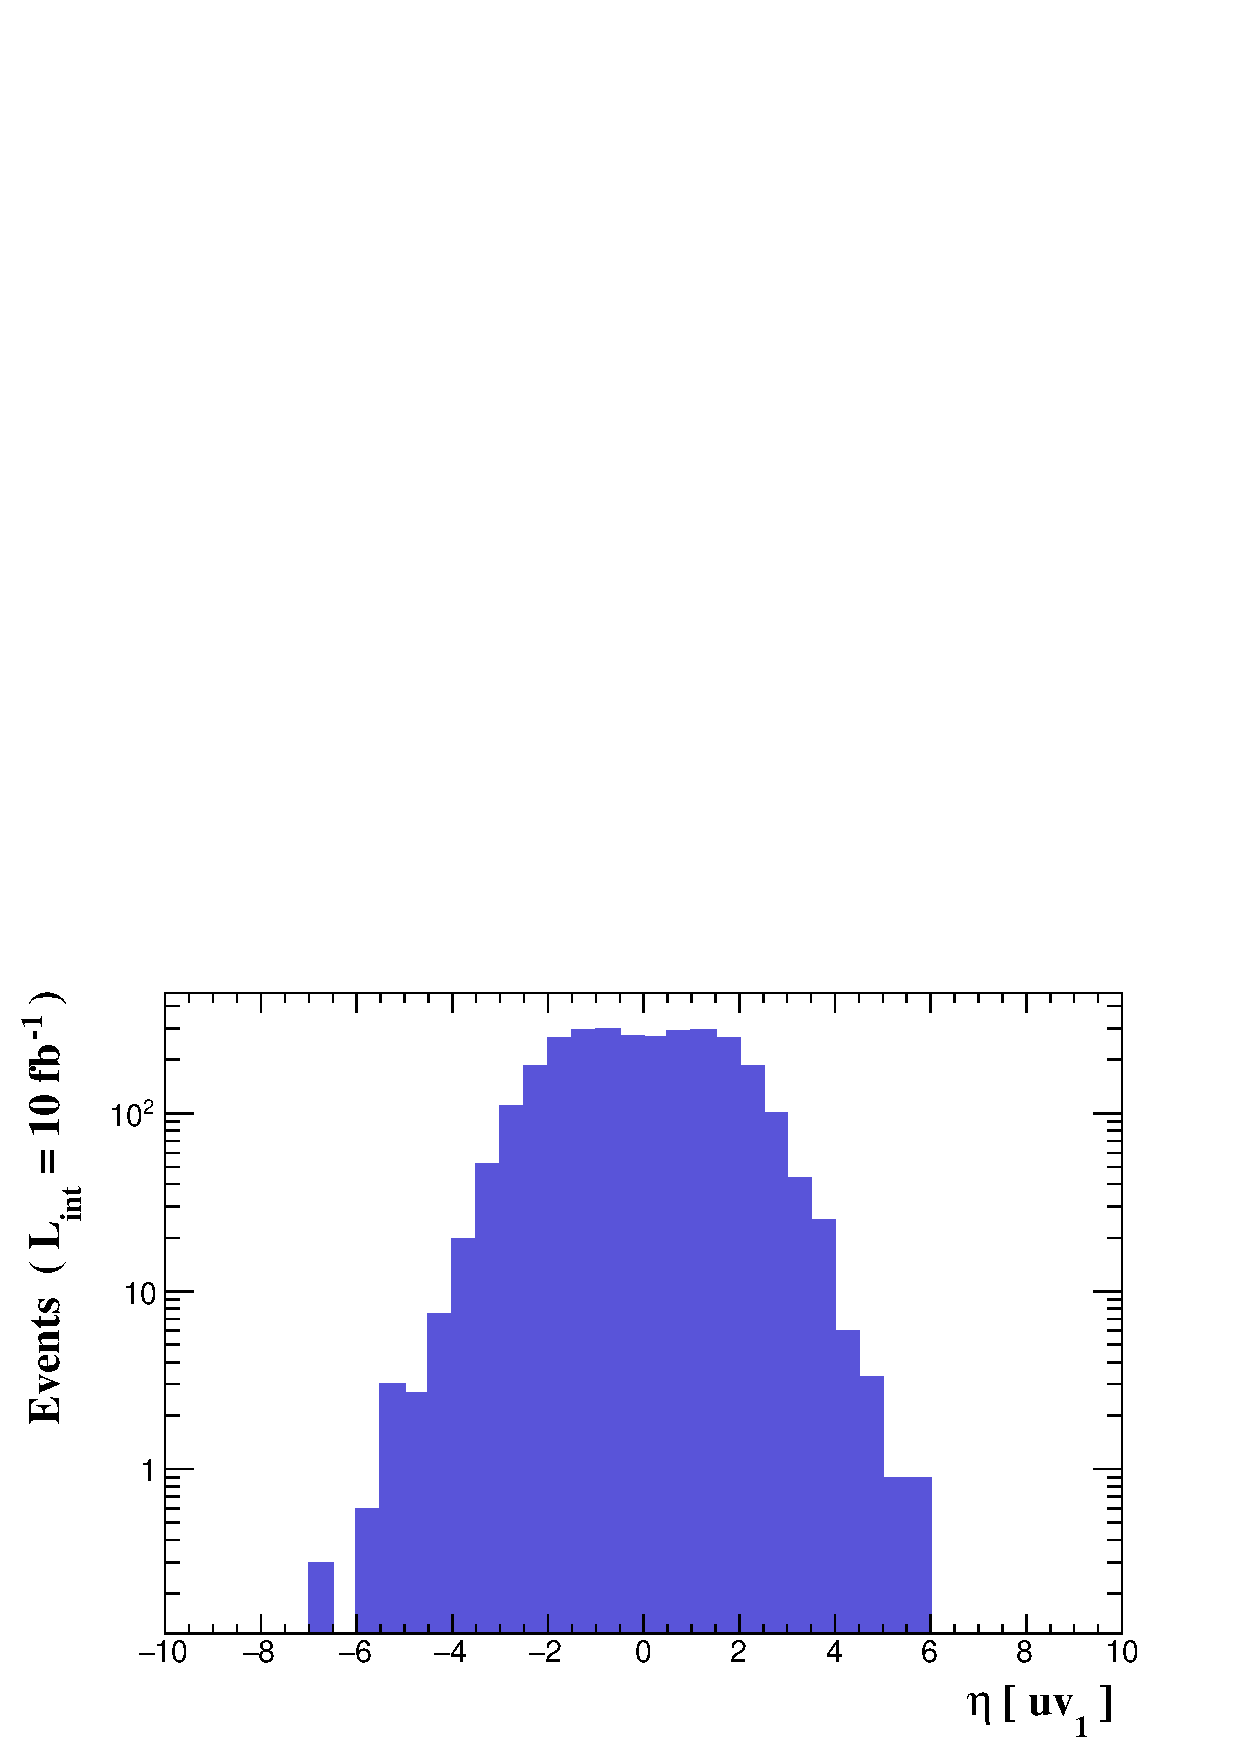
\includegraphics[scale=0.45]{selection_4.png}\\
\caption{   }
  \end{center}
\end{figure}
      \newpage
\subsection{ Histogram 6}

\textbf{* Plot: PT ( uv~[1] ) }\\
   \begin{table}[H]
  \begin{center}
    \begin{tabular}{|m{23.0mm}|m{23.0mm}|m{18.0mm}|m{19.0mm}|m{19.0mm}|m{19.0mm}|m{19.0mm}|}
      \hline
      {\cellcolor{yellow}         Dataset}& {\cellcolor{yellow}         Integral}& {\cellcolor{yellow}         Entries per event}& {\cellcolor{yellow}         Mean}& {\cellcolor{yellow}         RMS}& {\cellcolor{yellow}         \% underflow}& {\cellcolor{yellow}         \% overflow}\\
      \hline
      {\cellcolor{white}         unweighted\_events}& {\cellcolor{white}         2982}& {\cellcolor{white}         1.0}& {\cellcolor{white}         251.371}& {\cellcolor{white}         157.0}& {\cellcolor{orange}         0.0}& {\cellcolor{orange}         6.98}\\
\hline
    \end{tabular}
  \end{center}
\end{table}

\begin{figure}[H]
  \begin{center}
    \includegraphics[scale=0.45]{selection_5.png}\\
\caption{   }
  \end{center}
\end{figure}
      \newpage
\subsection{ Histogram 7}

\textbf{* Plot: ETA ( uv~[1] ) }\\
   \begin{table}[H]
  \begin{center}
    \begin{tabular}{|m{23.0mm}|m{23.0mm}|m{18.0mm}|m{19.0mm}|m{19.0mm}|m{19.0mm}|m{19.0mm}|}
      \hline
      {\cellcolor{yellow}         Dataset}& {\cellcolor{yellow}         Integral}& {\cellcolor{yellow}         Entries per event}& {\cellcolor{yellow}         Mean}& {\cellcolor{yellow}         RMS}& {\cellcolor{yellow}         \% underflow}& {\cellcolor{yellow}         \% overflow}\\
      \hline
      {\cellcolor{white}         unweighted\_events}& {\cellcolor{white}         2982}& {\cellcolor{white}         1.0}& {\cellcolor{white}         -0.0303749}& {\cellcolor{white}         1.697}& {\cellcolor{green}         0.0}& {\cellcolor{green}         0.0}\\
\hline
    \end{tabular}
  \end{center}
\end{table}

\begin{figure}[H]
  \begin{center}
    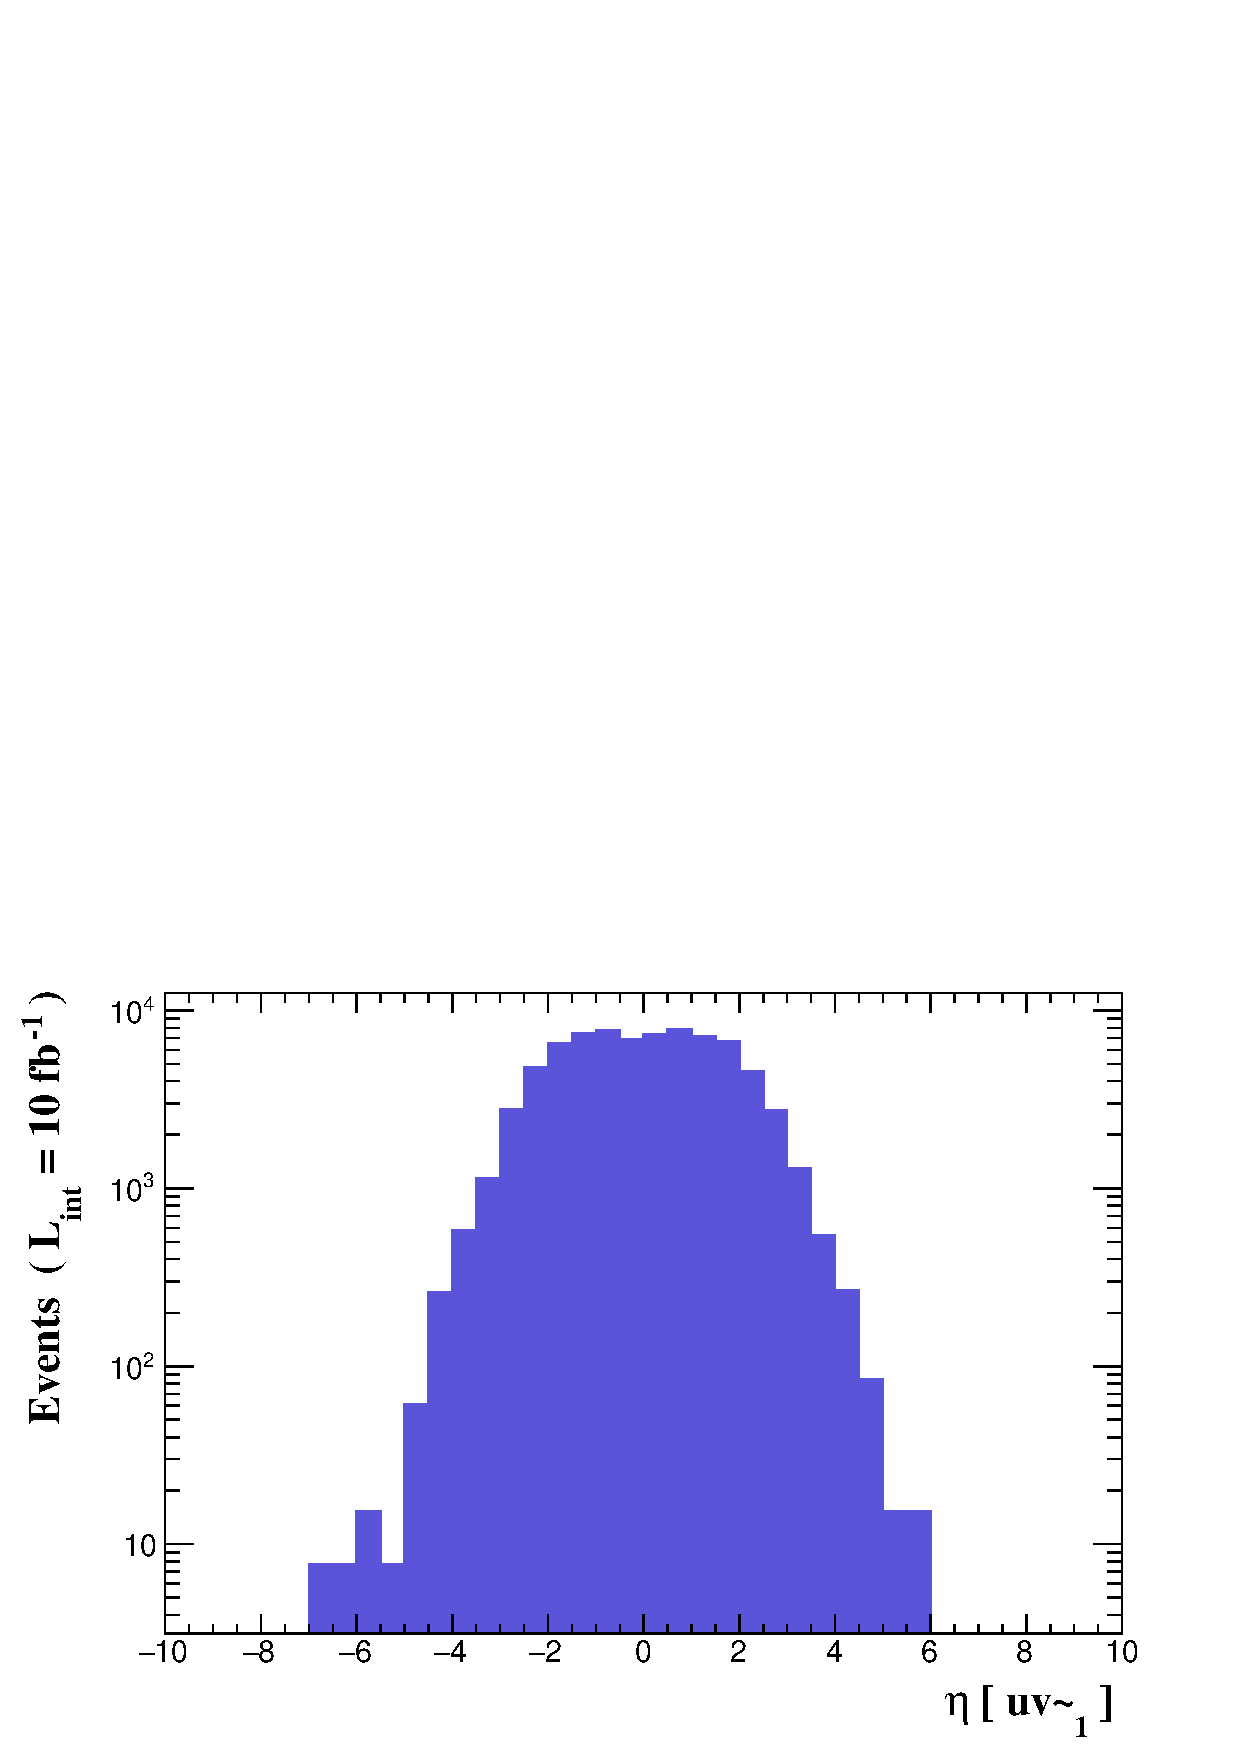
\includegraphics[scale=0.45]{selection_6.png}\\
\caption{   }
  \end{center}
\end{figure}
      \newpage
\subsection{ Histogram 8}

\textbf{* Plot: M ( uv[1] uv~[1] ) }\\
   \begin{table}[H]
  \begin{center}
    \begin{tabular}{|m{23.0mm}|m{23.0mm}|m{18.0mm}|m{19.0mm}|m{19.0mm}|m{19.0mm}|m{19.0mm}|}
      \hline
      {\cellcolor{yellow}         Dataset}& {\cellcolor{yellow}         Integral}& {\cellcolor{yellow}         Entries per event}& {\cellcolor{yellow}         Mean}& {\cellcolor{yellow}         RMS}& {\cellcolor{yellow}         \% underflow}& {\cellcolor{yellow}         \% overflow}\\
      \hline
      {\cellcolor{white}         unweighted\_events}& {\cellcolor{white}         2982}& {\cellcolor{white}         1.0}& {\cellcolor{white}         1122.71}& {\cellcolor{white}         302.3}& {\cellcolor{red}         0.0}& {\cellcolor{red}         100.0}\\
\hline
    \end{tabular}
  \end{center}
\end{table}

\begin{figure}[H]
  \begin{center}
    \includegraphics[scale=0.45]{selection_7.png}\\
\caption{   }
  \end{center}
\end{figure}
      \newpage
\subsection{ Histogram 9}

\textbf{* Plot: DELTAR ( uv[1] , uv~[1] ) }\\
   \begin{table}[H]
  \begin{center}
    \begin{tabular}{|m{23.0mm}|m{23.0mm}|m{18.0mm}|m{19.0mm}|m{19.0mm}|m{19.0mm}|m{19.0mm}|}
      \hline
      {\cellcolor{yellow}         Dataset}& {\cellcolor{yellow}         Integral}& {\cellcolor{yellow}         Entries per event}& {\cellcolor{yellow}         Mean}& {\cellcolor{yellow}         RMS}& {\cellcolor{yellow}         \% underflow}& {\cellcolor{yellow}         \% overflow}\\
      \hline
      {\cellcolor{white}         unweighted\_events}& {\cellcolor{white}         2982}& {\cellcolor{white}         1.0}& {\cellcolor{white}         3.57253}& {\cellcolor{white}         0.668}& {\cellcolor{green}         0.0}& {\cellcolor{green}         0.02}\\
\hline
    \end{tabular}
  \end{center}
\end{table}

\begin{figure}[H]
  \begin{center}
    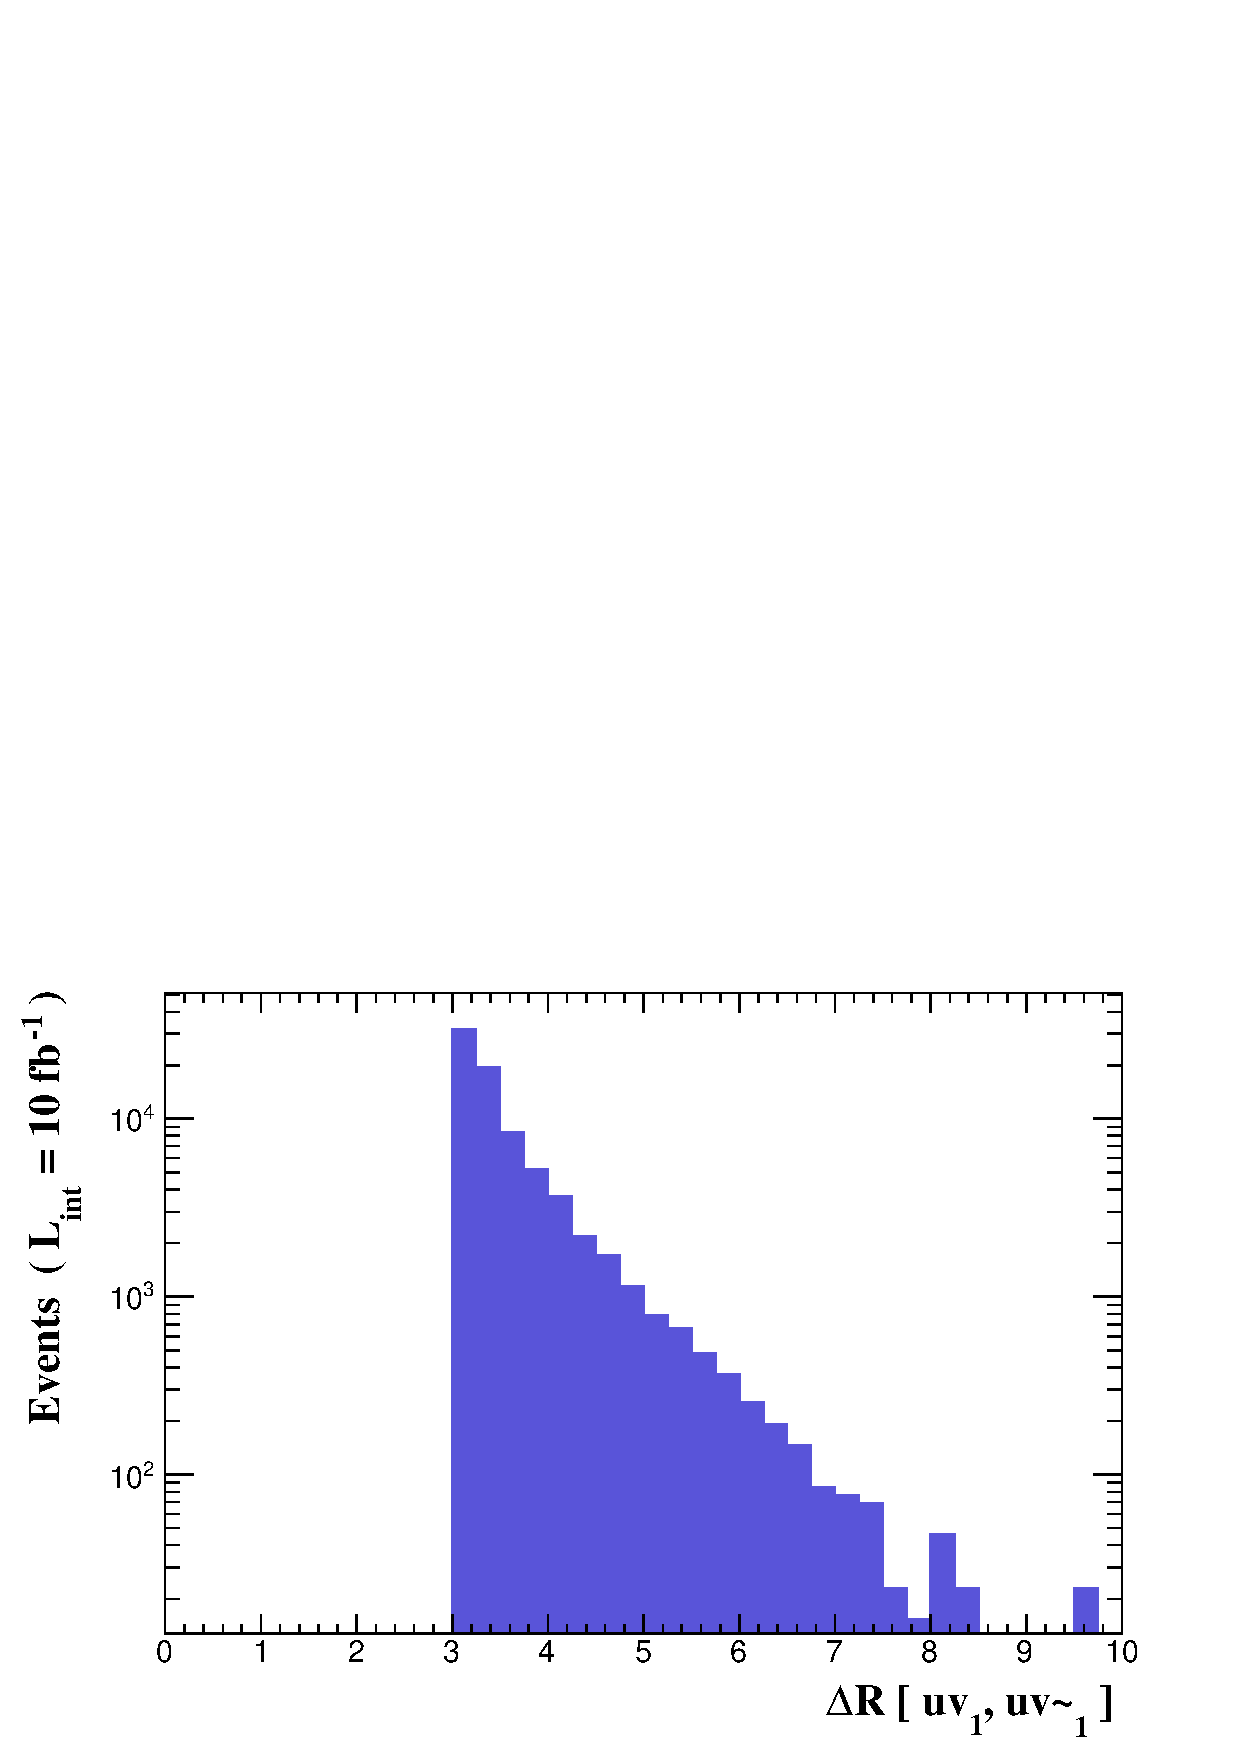
\includegraphics[scale=0.45]{selection_8.png}\\
\caption{   }
  \end{center}
\end{figure}
      \newpage
\subsection{ Histogram 10}

\textbf{* Plot: PT ( c[1] ) }\\
   \begin{table}[H]
  \begin{center}
    \begin{tabular}{|m{23.0mm}|m{23.0mm}|m{18.0mm}|m{19.0mm}|m{19.0mm}|m{19.0mm}|m{19.0mm}|}
      \hline
      {\cellcolor{yellow}         Dataset}& {\cellcolor{yellow}         Integral}& {\cellcolor{yellow}         Entries per event}& {\cellcolor{yellow}         Mean}& {\cellcolor{yellow}         RMS}& {\cellcolor{yellow}         \% underflow}& {\cellcolor{yellow}         \% overflow}\\
      \hline
      {\cellcolor{white}         unweighted\_events}& {\cellcolor{white}         2982}& {\cellcolor{white}         1.0}& {\cellcolor{white}         206.941}& {\cellcolor{white}         115.3}& {\cellcolor{green}         0.0}& {\cellcolor{green}         2.17}\\
\hline
    \end{tabular}
  \end{center}
\end{table}

\begin{figure}[H]
  \begin{center}
    \includegraphics[scale=0.45]{selection_9.png}\\
\caption{   }
  \end{center}
\end{figure}
      \newpage
\subsection{ Histogram 11}

\textbf{* Plot: ETA ( c[1] ) }\\
   \begin{table}[H]
  \begin{center}
    \begin{tabular}{|m{23.0mm}|m{23.0mm}|m{18.0mm}|m{19.0mm}|m{19.0mm}|m{19.0mm}|m{19.0mm}|}
      \hline
      {\cellcolor{yellow}         Dataset}& {\cellcolor{yellow}         Integral}& {\cellcolor{yellow}         Entries per event}& {\cellcolor{yellow}         Mean}& {\cellcolor{yellow}         RMS}& {\cellcolor{yellow}         \% underflow}& {\cellcolor{yellow}         \% overflow}\\
      \hline
      {\cellcolor{white}         unweighted\_events}& {\cellcolor{white}         2982}& {\cellcolor{white}         1.0}& {\cellcolor{white}         -0.0101637}& {\cellcolor{white}         1.271}& {\cellcolor{green}         0.0}& {\cellcolor{green}         0.0}\\
\hline
    \end{tabular}
  \end{center}
\end{table}

\begin{figure}[H]
  \begin{center}
    \includegraphics[scale=0.45]{selection_10.png}\\
\caption{   }
  \end{center}
\end{figure}
      \newpage
\subsection{ Histogram 12}

\textbf{* Plot: PT ( p1[1] ) }\\
   \begin{table}[H]
  \begin{center}
    \begin{tabular}{|m{23.0mm}|m{23.0mm}|m{18.0mm}|m{19.0mm}|m{19.0mm}|m{19.0mm}|m{19.0mm}|}
      \hline
      {\cellcolor{yellow}         Dataset}& {\cellcolor{yellow}         Integral}& {\cellcolor{yellow}         Entries per event}& {\cellcolor{yellow}         Mean}& {\cellcolor{yellow}         RMS}& {\cellcolor{yellow}         \% underflow}& {\cellcolor{yellow}         \% overflow}\\
      \hline
      {\cellcolor{white}         unweighted\_events}& {\cellcolor{white}         2982}& {\cellcolor{white}         1.0}& {\cellcolor{white}         207.339}& {\cellcolor{white}         114.3}& {\cellcolor{green}         0.0}& {\cellcolor{green}         2.18}\\
\hline
    \end{tabular}
  \end{center}
\end{table}

\begin{figure}[H]
  \begin{center}
    \includegraphics[scale=0.45]{selection_11.png}\\
\caption{   }
  \end{center}
\end{figure}
      \newpage
\subsection{ Histogram 13}

\textbf{* Plot: ETA ( p1[1] ) }\\
   \begin{table}[H]
  \begin{center}
    \begin{tabular}{|m{23.0mm}|m{23.0mm}|m{18.0mm}|m{19.0mm}|m{19.0mm}|m{19.0mm}|m{19.0mm}|}
      \hline
      {\cellcolor{yellow}         Dataset}& {\cellcolor{yellow}         Integral}& {\cellcolor{yellow}         Entries per event}& {\cellcolor{yellow}         Mean}& {\cellcolor{yellow}         RMS}& {\cellcolor{yellow}         \% underflow}& {\cellcolor{yellow}         \% overflow}\\
      \hline
      {\cellcolor{white}         unweighted\_events}& {\cellcolor{white}         2982}& {\cellcolor{white}         1.0}& {\cellcolor{white}         -0.0052323}& {\cellcolor{white}         1.275}& {\cellcolor{green}         0.0}& {\cellcolor{green}         0.0}\\
\hline
    \end{tabular}
  \end{center}
\end{table}

\begin{figure}[H]
  \begin{center}
    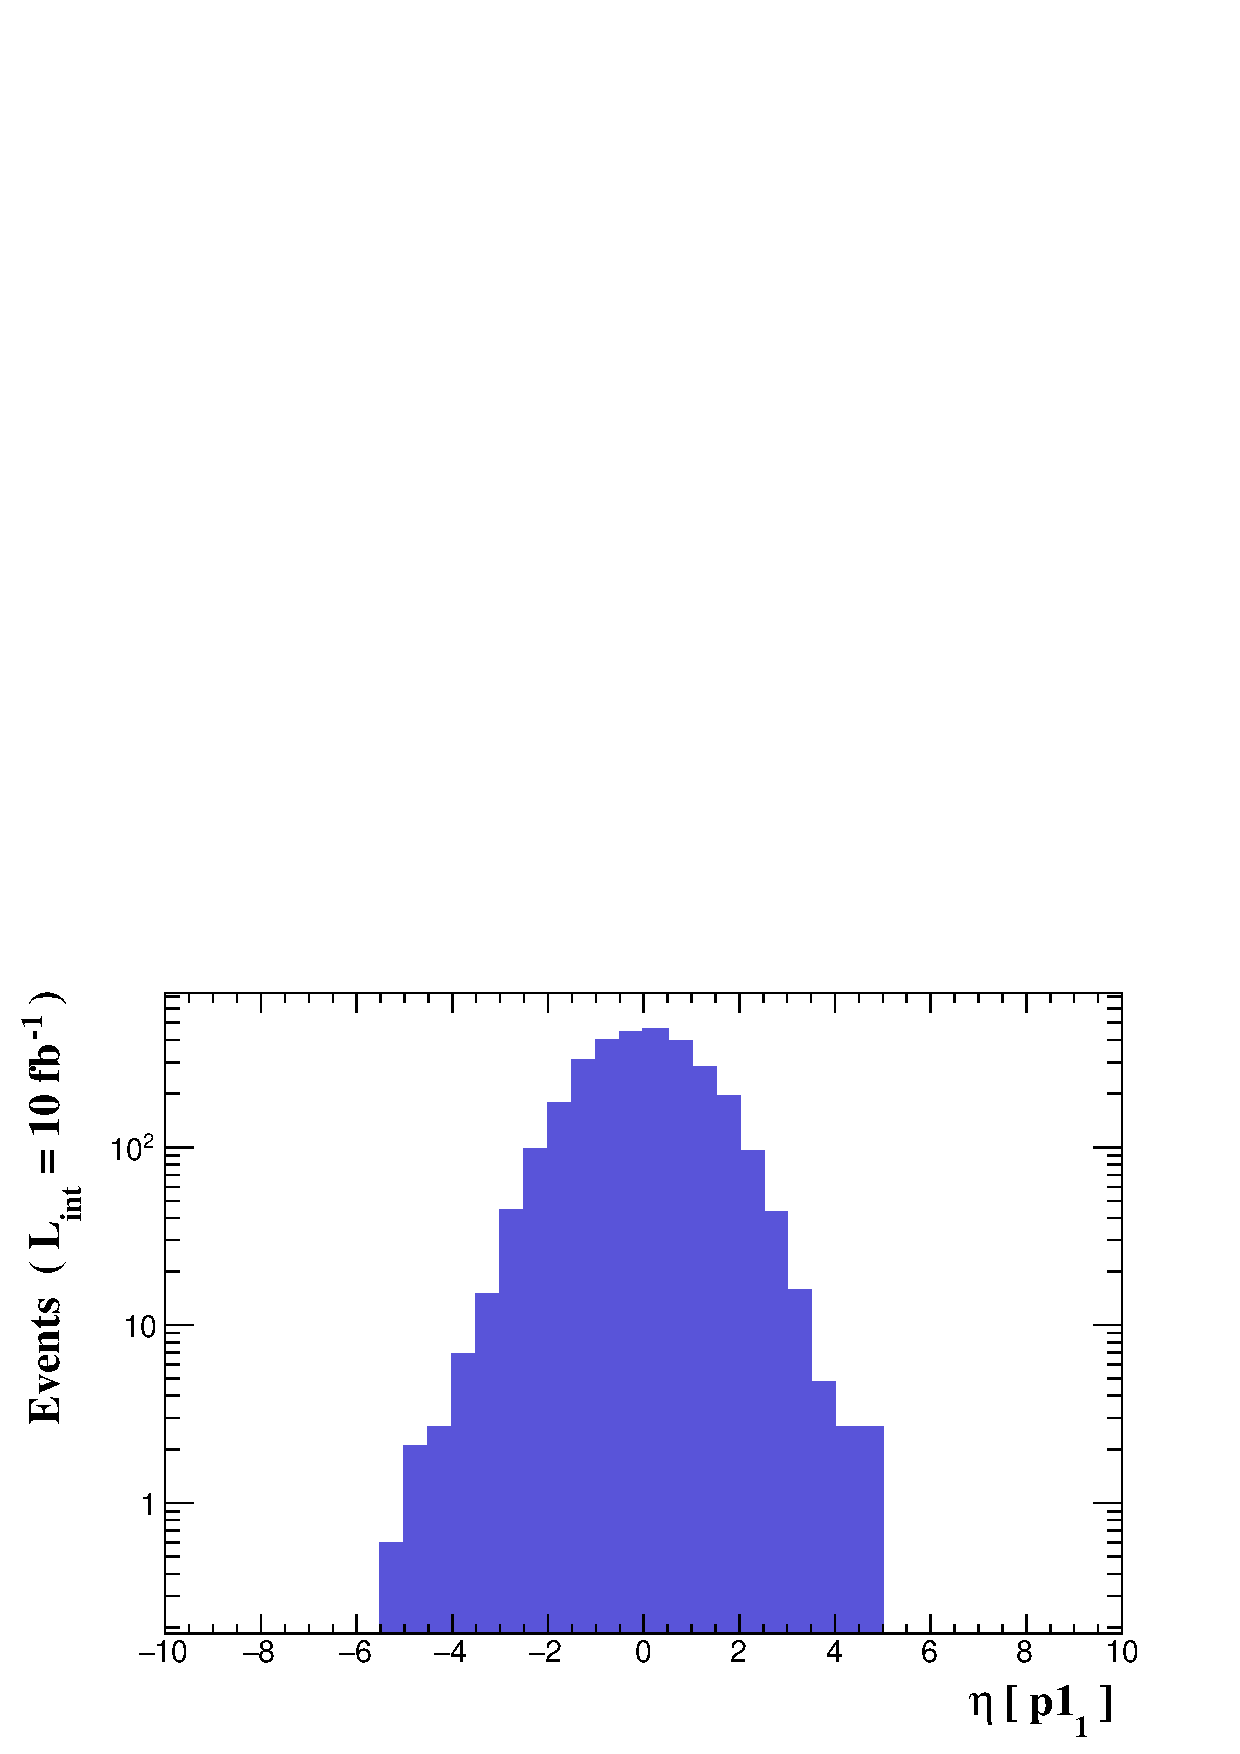
\includegraphics[scale=0.45]{selection_12.png}\\
\caption{   }
  \end{center}
\end{figure}
      \newpage
\subsection{ Histogram 14}

\textbf{* Plot: PT ( uv~[1] ) }\\
   \begin{table}[H]
  \begin{center}
    \begin{tabular}{|m{23.0mm}|m{23.0mm}|m{18.0mm}|m{19.0mm}|m{19.0mm}|m{19.0mm}|m{19.0mm}|}
      \hline
      {\cellcolor{yellow}         Dataset}& {\cellcolor{yellow}         Integral}& {\cellcolor{yellow}         Entries per event}& {\cellcolor{yellow}         Mean}& {\cellcolor{yellow}         RMS}& {\cellcolor{yellow}         \% underflow}& {\cellcolor{yellow}         \% overflow}\\
      \hline
      {\cellcolor{white}         unweighted\_events}& {\cellcolor{white}         2982}& {\cellcolor{white}         1.0}& {\cellcolor{white}         251.371}& {\cellcolor{white}         157.0}& {\cellcolor{orange}         0.0}& {\cellcolor{orange}         6.98}\\
\hline
    \end{tabular}
  \end{center}
\end{table}

\begin{figure}[H]
  \begin{center}
    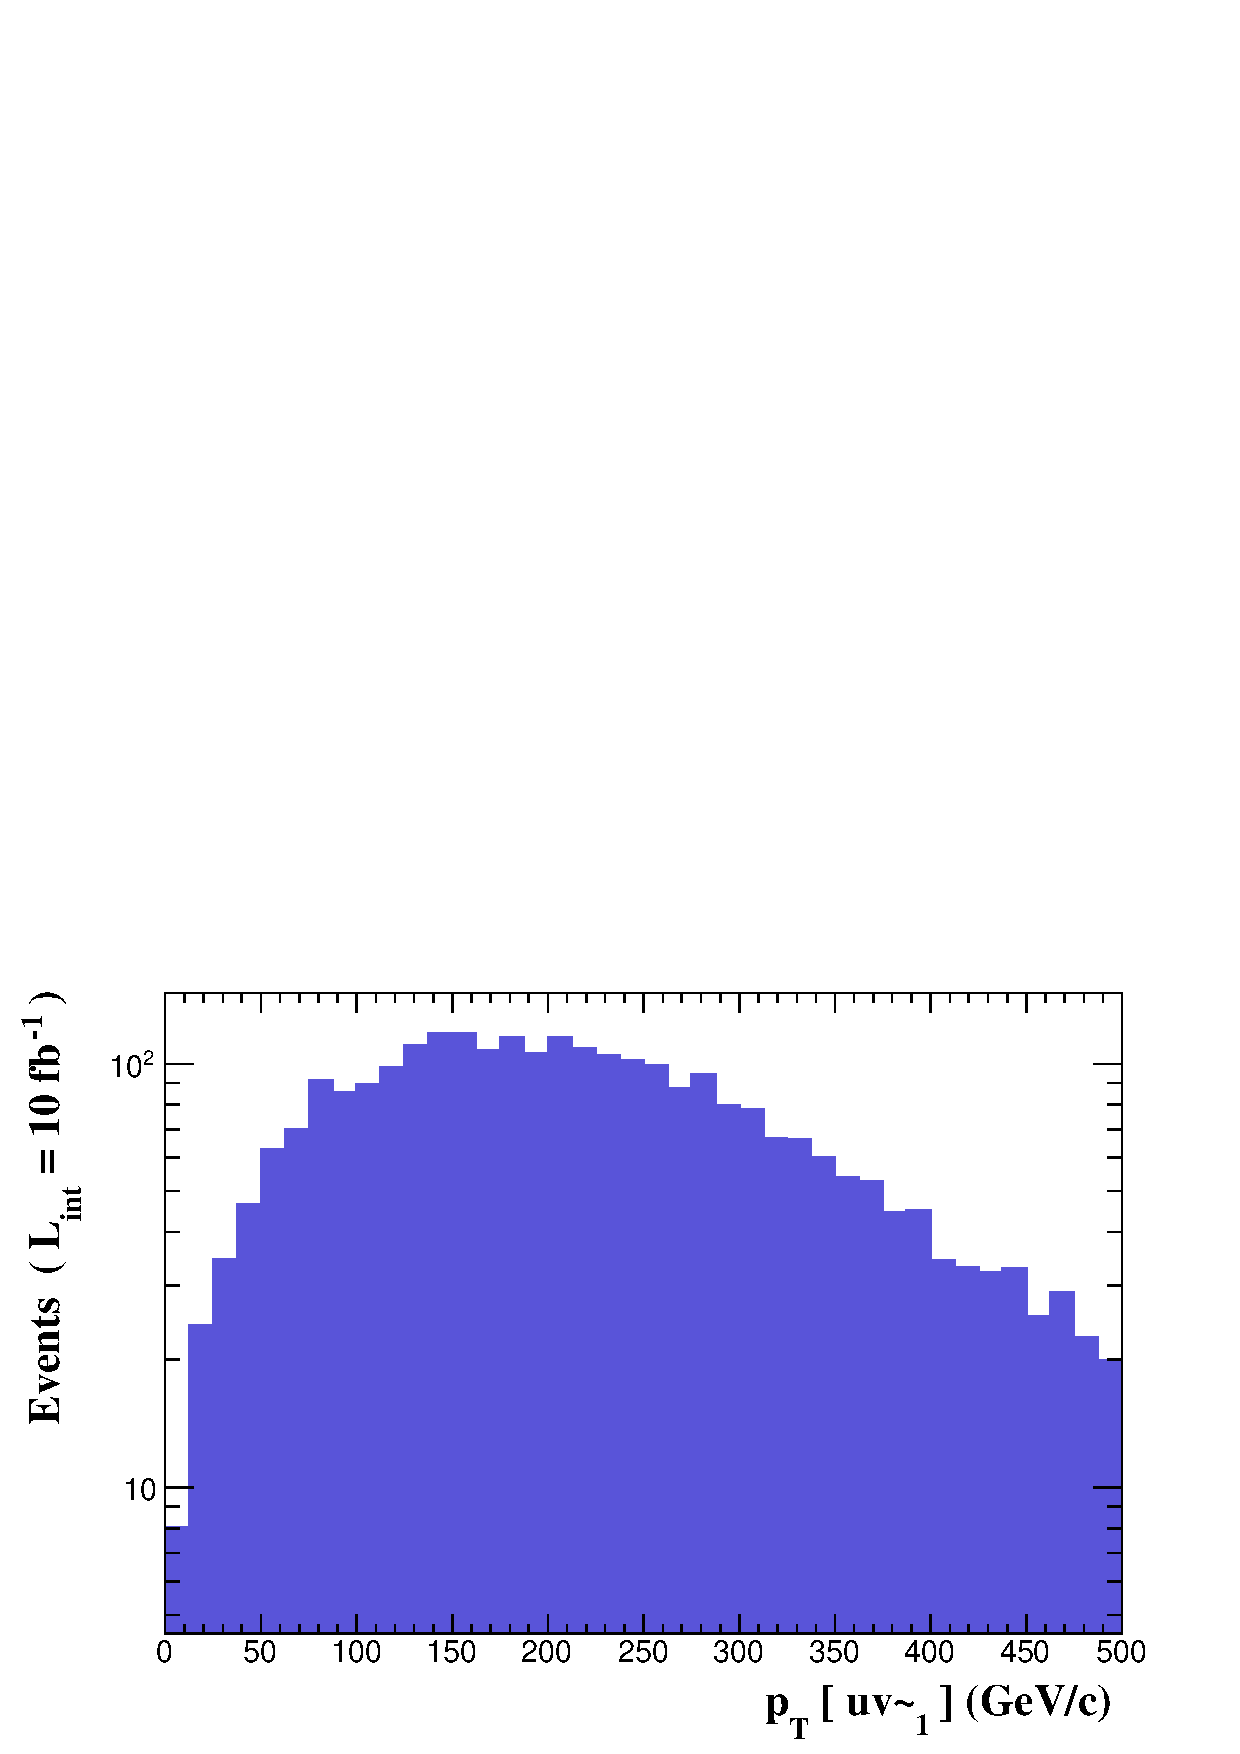
\includegraphics[scale=0.45]{selection_13.png}\\
\caption{   }
  \end{center}
\end{figure}
      \newpage
\subsection{ Histogram 15}

\textbf{* Plot: ETA ( uv~[1] ) }\\
   \begin{table}[H]
  \begin{center}
    \begin{tabular}{|m{23.0mm}|m{23.0mm}|m{18.0mm}|m{19.0mm}|m{19.0mm}|m{19.0mm}|m{19.0mm}|}
      \hline
      {\cellcolor{yellow}         Dataset}& {\cellcolor{yellow}         Integral}& {\cellcolor{yellow}         Entries per event}& {\cellcolor{yellow}         Mean}& {\cellcolor{yellow}         RMS}& {\cellcolor{yellow}         \% underflow}& {\cellcolor{yellow}         \% overflow}\\
      \hline
      {\cellcolor{white}         unweighted\_events}& {\cellcolor{white}         2982}& {\cellcolor{white}         1.0}& {\cellcolor{white}         -0.0303749}& {\cellcolor{white}         1.697}& {\cellcolor{green}         0.0}& {\cellcolor{green}         0.0}\\
\hline
    \end{tabular}
  \end{center}
\end{table}

\begin{figure}[H]
  \begin{center}
    \includegraphics[scale=0.45]{selection_14.png}\\
\caption{   }
  \end{center}
\end{figure}
      \newpage
\subsection{ Histogram 16}

\textbf{* Plot: M ( c[1] p1[1] ) }\\
   \begin{table}[H]
  \begin{center}
    \begin{tabular}{|m{23.0mm}|m{23.0mm}|m{18.0mm}|m{19.0mm}|m{19.0mm}|m{19.0mm}|m{19.0mm}|}
      \hline
      {\cellcolor{yellow}         Dataset}& {\cellcolor{yellow}         Integral}& {\cellcolor{yellow}         Entries per event}& {\cellcolor{yellow}         Mean}& {\cellcolor{yellow}         RMS}& {\cellcolor{yellow}         \% underflow}& {\cellcolor{yellow}         \% overflow}\\
      \hline
      {\cellcolor{white}         unweighted\_events}& {\cellcolor{white}         2982}& {\cellcolor{white}         1.0}& {\cellcolor{white}         399.97}& {\cellcolor{white}         2.149}& {\cellcolor{green}         0.0}& {\cellcolor{green}         0.0}\\
\hline
    \end{tabular}
  \end{center}
\end{table}

\begin{figure}[H]
  \begin{center}
    \includegraphics[scale=0.45]{selection_15.png}\\
\caption{   }
  \end{center}
\end{figure}
      \newpage
\subsection{ Histogram 17}

\textbf{* Plot: M ( c[1] p1[1] uv~[1] ) }\\
   \begin{table}[H]
  \begin{center}
    \begin{tabular}{|m{23.0mm}|m{23.0mm}|m{18.0mm}|m{19.0mm}|m{19.0mm}|m{19.0mm}|m{19.0mm}|}
      \hline
      {\cellcolor{yellow}         Dataset}& {\cellcolor{yellow}         Integral}& {\cellcolor{yellow}         Entries per event}& {\cellcolor{yellow}         Mean}& {\cellcolor{yellow}         RMS}& {\cellcolor{yellow}         \% underflow}& {\cellcolor{yellow}         \% overflow}\\
      \hline
      {\cellcolor{white}         unweighted\_events}& {\cellcolor{white}         2982}& {\cellcolor{white}         1.0}& {\cellcolor{white}         1122.71}& {\cellcolor{white}         302.3}& {\cellcolor{red}         0.0}& {\cellcolor{red}         100.0}\\
\hline
    \end{tabular}
  \end{center}
\end{table}

\begin{figure}[H]
  \begin{center}
    \includegraphics[scale=0.45]{selection_16.png}\\
\caption{   }
  \end{center}
\end{figure}
      \newpage
\subsection{ Histogram 18}

\textbf{* Plot: M ( c[1] uv~[1] ) }\\
   \begin{table}[H]
  \begin{center}
    \begin{tabular}{|m{23.0mm}|m{23.0mm}|m{18.0mm}|m{19.0mm}|m{19.0mm}|m{19.0mm}|m{19.0mm}|}
      \hline
      {\cellcolor{yellow}         Dataset}& {\cellcolor{yellow}         Integral}& {\cellcolor{yellow}         Entries per event}& {\cellcolor{yellow}         Mean}& {\cellcolor{yellow}         RMS}& {\cellcolor{yellow}         \% underflow}& {\cellcolor{yellow}         \% overflow}\\
      \hline
      {\cellcolor{white}         unweighted\_events}& {\cellcolor{white}         2982}& {\cellcolor{white}         1.0}& {\cellcolor{white}         774.79}& {\cellcolor{white}         271.2}& {\cellcolor{red}         0.0}& {\cellcolor{red}         93.86}\\
\hline
    \end{tabular}
  \end{center}
\end{table}

\begin{figure}[H]
  \begin{center}
    \includegraphics[scale=0.45]{selection_17.png}\\
\caption{   }
  \end{center}
\end{figure}
      \newpage
\subsection{ Histogram 19}

\textbf{* Plot: M ( p1[1] uv~[1] ) }\\
   \begin{table}[H]
  \begin{center}
    \begin{tabular}{|m{23.0mm}|m{23.0mm}|m{18.0mm}|m{19.0mm}|m{19.0mm}|m{19.0mm}|m{19.0mm}|}
      \hline
      {\cellcolor{yellow}         Dataset}& {\cellcolor{yellow}         Integral}& {\cellcolor{yellow}         Entries per event}& {\cellcolor{yellow}         Mean}& {\cellcolor{yellow}         RMS}& {\cellcolor{yellow}         \% underflow}& {\cellcolor{yellow}         \% overflow}\\
      \hline
      {\cellcolor{white}         unweighted\_events}& {\cellcolor{white}         2982}& {\cellcolor{white}         1.0}& {\cellcolor{white}         777.706}& {\cellcolor{white}         270.5}& {\cellcolor{red}         0.0}& {\cellcolor{red}         94.06}\\
\hline
    \end{tabular}
  \end{center}
\end{table}

\begin{figure}[H]
  \begin{center}
    \includegraphics[scale=0.45]{selection_18.png}\\
\caption{   }
  \end{center}
\end{figure}
      \newpage
\subsection{ Histogram 20}

\textbf{* Plot: DELTAR ( c[1] , p1[1] ) }\\
   \begin{table}[H]
  \begin{center}
    \begin{tabular}{|m{23.0mm}|m{23.0mm}|m{18.0mm}|m{19.0mm}|m{19.0mm}|m{19.0mm}|m{19.0mm}|}
      \hline
      {\cellcolor{yellow}         Dataset}& {\cellcolor{yellow}         Integral}& {\cellcolor{yellow}         Entries per event}& {\cellcolor{yellow}         Mean}& {\cellcolor{yellow}         RMS}& {\cellcolor{yellow}         \% underflow}& {\cellcolor{yellow}         \% overflow}\\
      \hline
      {\cellcolor{white}         unweighted\_events}& {\cellcolor{white}         2982}& {\cellcolor{white}         1.0}& {\cellcolor{white}         2.61548}& {\cellcolor{white}         0.6749}& {\cellcolor{green}         0.0}& {\cellcolor{green}         0.0}\\
\hline
    \end{tabular}
  \end{center}
\end{table}

\begin{figure}[H]
  \begin{center}
    \includegraphics[scale=0.45]{selection_19.png}\\
\caption{   }
  \end{center}
\end{figure}
      \newpage
\subsection{ Histogram 21}

\textbf{* Plot: DELTAR ( c[1] , uv~[1] ) }\\
   \begin{table}[H]
  \begin{center}
    \begin{tabular}{|m{23.0mm}|m{23.0mm}|m{18.0mm}|m{19.0mm}|m{19.0mm}|m{19.0mm}|m{19.0mm}|}
      \hline
      {\cellcolor{yellow}         Dataset}& {\cellcolor{yellow}         Integral}& {\cellcolor{yellow}         Entries per event}& {\cellcolor{yellow}         Mean}& {\cellcolor{yellow}         RMS}& {\cellcolor{yellow}         \% underflow}& {\cellcolor{yellow}         \% overflow}\\
      \hline
      {\cellcolor{white}         unweighted\_events}& {\cellcolor{white}         2982}& {\cellcolor{white}         1.0}& {\cellcolor{white}         2.72079}& {\cellcolor{white}         0.9118}& {\cellcolor{green}         0.0}& {\cellcolor{green}         0.0}\\
\hline
    \end{tabular}
  \end{center}
\end{table}

\begin{figure}[H]
  \begin{center}
    \includegraphics[scale=0.45]{selection_20.png}\\
\caption{   }
  \end{center}
\end{figure}
      \newpage
\subsection{ Histogram 22}

\textbf{* Plot: DELTAR ( p1[1] , uv~[1] ) }\\
   \begin{table}[H]
  \begin{center}
    \begin{tabular}{|m{23.0mm}|m{23.0mm}|m{18.0mm}|m{19.0mm}|m{19.0mm}|m{19.0mm}|m{19.0mm}|}
      \hline
      {\cellcolor{yellow}         Dataset}& {\cellcolor{yellow}         Integral}& {\cellcolor{yellow}         Entries per event}& {\cellcolor{yellow}         Mean}& {\cellcolor{yellow}         RMS}& {\cellcolor{yellow}         \% underflow}& {\cellcolor{yellow}         \% overflow}\\
      \hline
      {\cellcolor{white}         unweighted\_events}& {\cellcolor{white}         2982}& {\cellcolor{white}         1.0}& {\cellcolor{white}         2.7398}& {\cellcolor{white}         0.903}& {\cellcolor{green}         0.0}& {\cellcolor{green}         0.0}\\
\hline
    \end{tabular}
  \end{center}
\end{table}

\begin{figure}[H]
  \begin{center}
    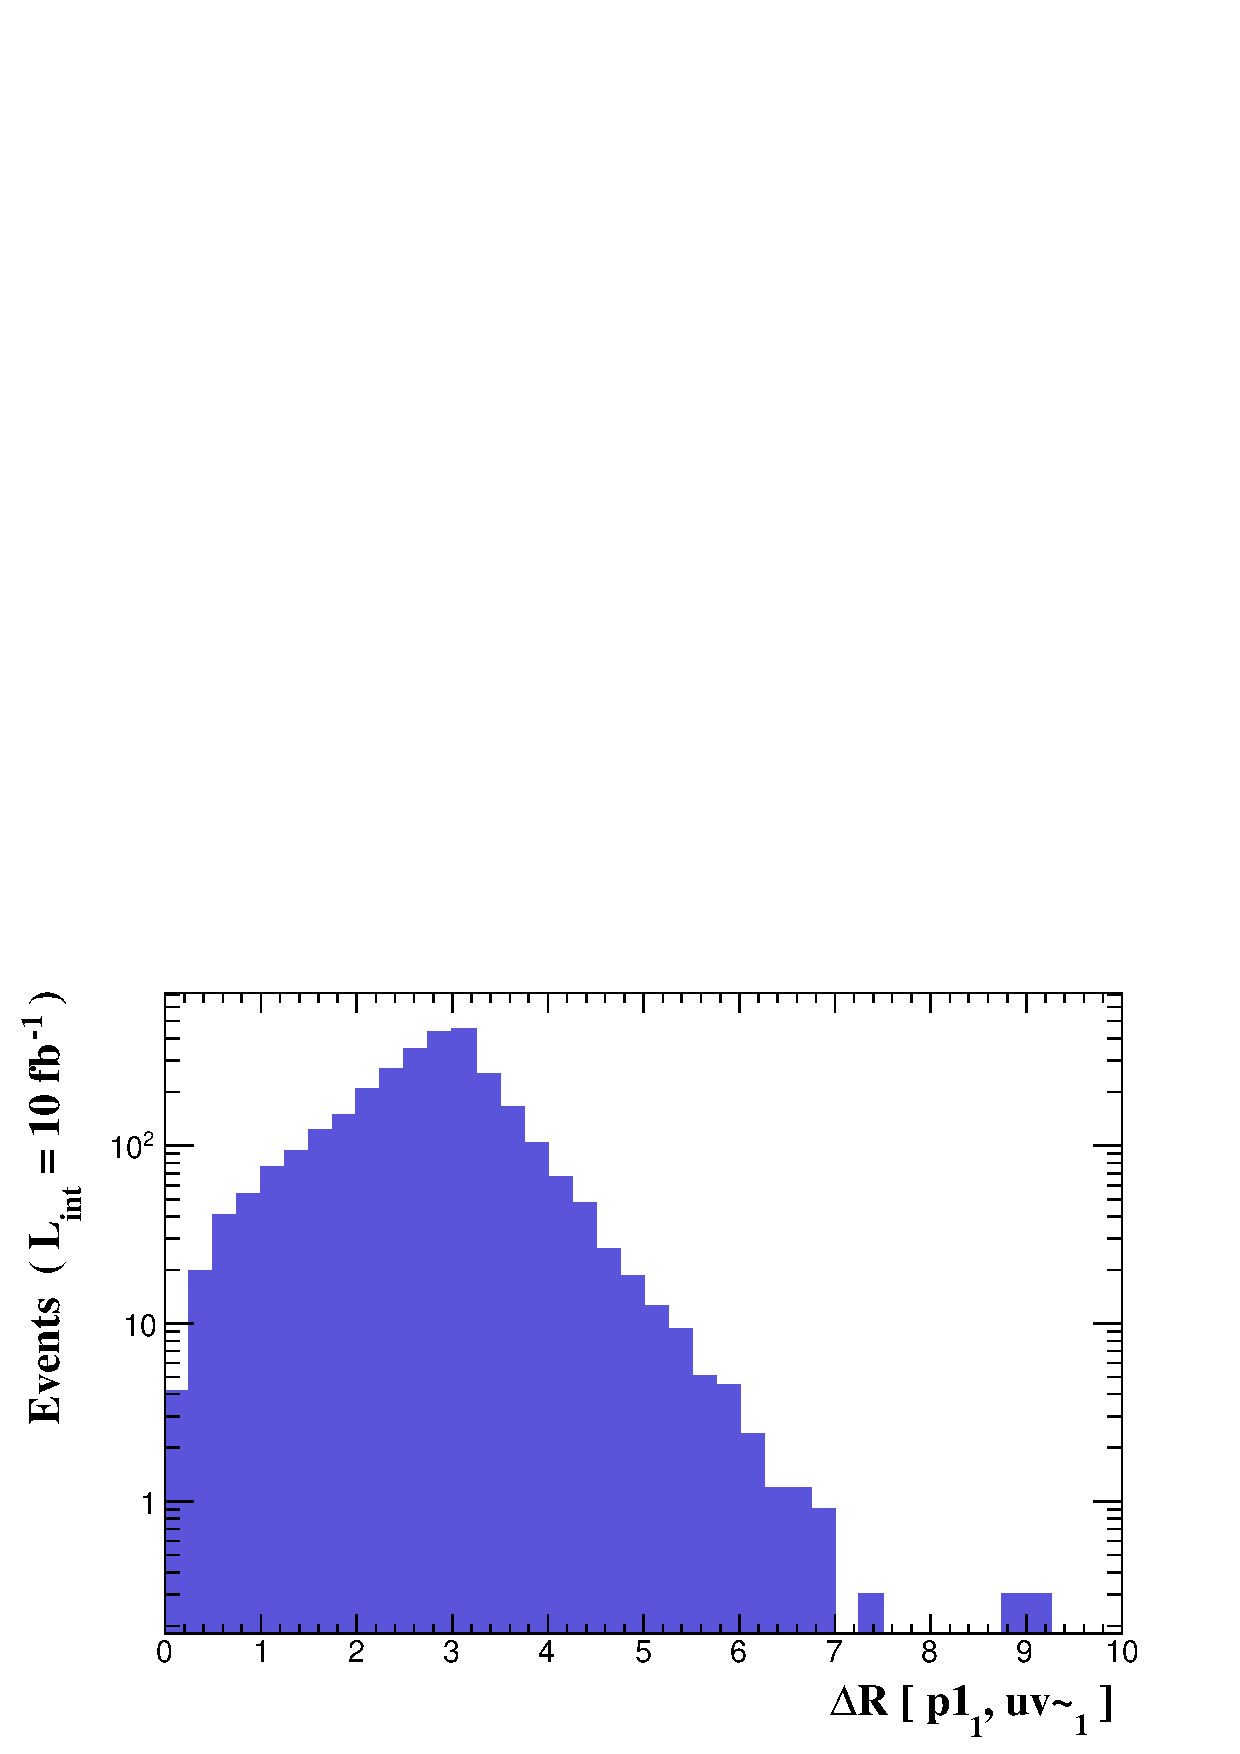
\includegraphics[scale=0.45]{selection_21.png}\\
\caption{   }
  \end{center}
\end{figure}
      \end{document}
